\subsubsection{09.02.15}
\begin{enumerate}
	
	\item Время начала и окончания собрания: 16:10 - 22:00.
	
	\item Цели собрания: 
	\begin{enumerate}
		
		\item Реализовать защиту колес от наезда на мячи и палку-упор. 
		
		\item Упаковать робота для поездки на центральный робофест, который пройдет 11-13 февраля в Москве.
		
	\end{enumerate}

	\item Проделанная работа:
	\begin{enumerate}
		
		\item Поскольку сбоку у робота защита от мячей уже имелась, а сзади от наезда на палку-упор его будет предохранять подвижная корзина, было решено установить защиту только спереди. Уголки, защищающие робота от наезда на палку и мячи, были установлены таким образом, чтобы не мешать роботу заезжать на пандус.
		\begin{figure}[H]
			\begin{minipage}[h]{0.4\linewidth}
				\center{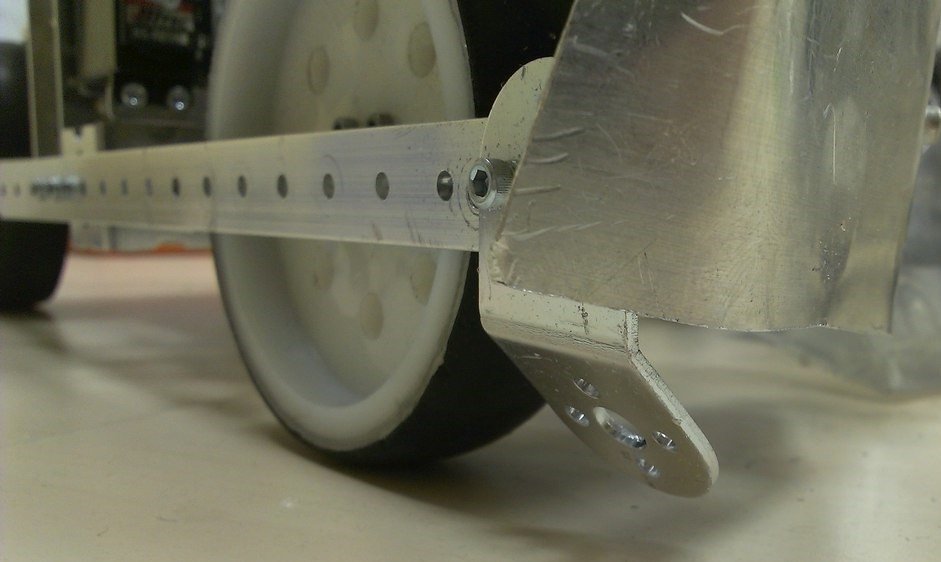
\includegraphics[scale=0.2]{days/09.02.15/images/01}}
			\end{minipage}
			\hfill
			\begin{minipage}[h]{0.55\linewidth}
				\center{
\includegraphics[scale=0.23]{days/09.02.15/images/02}}
			\end{minipage}
			\caption{Защита от палки}
		\end{figure}
		
		\item В конце занятия робот был упакован в коробку и подготовлен к транспортировке.
		
	\end{enumerate}
	
	\item Итоги собрания:
	\begin{enumerate}
		
		\item Защита колес от палки-упора установлена.
		
		\item Робот готов к транспортировке на соревнования.
		
	\end{enumerate}
	
	\item Задачи для последующих собраний:
	\begin{enumerate}
		
		\item Выступить на соревнованиях в Москве как можно лучше.
			
	\end{enumerate}
\end{enumerate}
\fillpage
